\documentclass[runningheads]{llncs}
\usepackage[spanish]{babel}
\usepackage{todonotes}
\usepackage{amsmath}
\usepackage{graphicx}
\usepackage{url}
\usepackage{hyperref} % Paquete para enlaces clicables
\usepackage{array}
\usepackage{subcaption}

\newcommand{\keywords}[1]{\\ \\ \textbf{Palabras clave:} #1}
\begin{document}

\title{Sistema de Recomendación Secuencial usando Redes Neuronales Recursivas}
\author{Jackson Vera Pineda \\ Kevin Manzano Rodríguez \\ Roger Fuentes Rodríguez}
\institute{\url{https://github.com/jackverneda/sri-summer-2024}}


\selectlanguage{spanish}
\maketitle

\begin{abstract}
Este informe describe la implementación de un sistema de recomendación secuencial basado en redes neuronales recurrentes (RNN) utilizando capas LSTM (Long Short-Term Memory) y GRU (Gated Recurrent Units) haciendo uso además de modelos de lenguaje para capturar la semántica de los productos en embeddings. Este sistema tiene como objetivo predecir el siguiente producto en el que un usuario podría estar interesado, basándose en sus interacciones anteriores.
\keywords{Recomendación secuencial, Redes Neuronales Recursivas, LSTM, GRU, Deep Learning}
\end{abstract}


\section{Introducción}

\space En la era del comercio electrónico y las plataformas de contenido, la capacidad de ofrecer recomendaciones personalizadas a los usuarios se ha convertido en un factor crucial para mejorar la experiencia del usuario y aumentar la retención. Un enfoque efectivo es predecir el siguiente producto que un usuario podría interactuar basándose en su historial de interacciones pasadas. Este problema se conoce como ``recomendación secuencial", donde el objetivo es utilizar secuencias temporales de interacciones de usuarios para predecir sus futuras acciones.

El desafío principal en la recomendación secuencial es capturar las dependencias temporales y la evolución de las preferencias de los usuarios a lo largo del tiempo. Las Redes Neuronales Recursivas (RNN) y sus variantes, como LSTM (\textit{Long Short-Term Memory}) y GRU (\textit{Gated Recurrent Units}), han demostrado ser herramientas poderosas para modelar secuencias temporales debido a su capacidad para retener y procesar información a través de secuencias largas.

\section{Formulación del Problema}

Para desarrollar un modelo de recomendación secuencial en este proyecto académico, se optó por diseñar una problemática específica dentro de un escenario ficticio pero representativo de una situación real. Este enfoque permite que cada componente del problema y su solución sean detalladamente especificados dentro del contexto planteado, facilitando así la explicación del proyecto. No obstante, es importante señalar que tanto la problemática como la solución propuestas son generalizables a muchos escenarios similares.

El caso ficticio trata sobre una tienda online de cosméticos que requiere un sistema de recomendación capaz de sugerir productos de interés personal a sus usuarios en el futuro. Este desafío se complica debido a la gran cantidad de productos disponibles y al crecimiento constante de su base de datos (nuevo clientes y más compras). Actualmente, la tienda utiliza un sistema de búsqueda por coincidencias, y no considera sugerencias creativas ni personalizadas. Además, en esta se registra cada compra realizada por los usuarios, y se dispone como fuente de datos valiosa para implementar el sistema de recomendación.

\section{Propuesta de la Solución}

Entre las soluciones más destacadas para modelar problemas de recomendación secuencial se encuentran: Modelos Basados en Redes Neuronales Recurrentes (RNNs), Modelos de Atención \cite{kang2018self}, Modelos Basados en Grafos \cite{escamillasistema} y Modelos de Aprendizaje por Refuerzo \cite{ali2024analyzing}.

En particular, los Modelos Basados en Redes Neuronales Recurrentes han demostrado ser altamente eficaces para capturar las dependencias temporales en secuencias de datos, lo que los convierte en una opción adecuada para sistemas de recomendación secuencial \cite{goodfellow2016deep}. Un ejemplo notable es el trabajo de Hidasi et al., donde se emplean RNNs para recomendaciones basadas en sesiones \cite{hidasi2016session}. Este enfoque utiliza variantes como Gated Recurrent Units (GRU) para mejorar la precisión de las recomendaciones a partir del historial de interacciones de los usuarios. Además, estudios empíricos han demostrado que las GRU pueden superar en rendimiento a las LSTM en ciertos contextos de modelado secuencial \cite{chung2014empirical}.

En este trabajo, proponemos un enfoque similar al de Hidasi et al. \cite{hidasi2016session}, pero con varias mejoras. La principal diferencia radica en que, en lugar de usar directamente el ID del producto como entrada a la red neuronal, proponemos transformarlo en un vector de mayor dimensión dentro de un espacio de productos. En este espacio, las relaciones implícitas entre productos se representan mediante la cercanía de los vectores; es decir, cuanto menor sea la distancia entre dos vectores, mayor será la relación entre los productos que representan.

Para la problemática de este trabajo, la semántica de este espacio vectorial está determinada por los nombres de los productos, lo que permite que se asemeje al lenguaje natural. Por lo tanto bastará con seleccionar un Modelo de Embeddings entrenado para transformar oraciones de lenguaje natural a vectores numéricos de alguna dimensión.

Este enfoque se distingue ligeramente de otros trabajos como \cite{chung2014empirical,tang2018personalized}, donde los embeddings de los IDs de los productos se generan dentro de la red neuronal en las primeras capas, comúnmente denominadas Capas de Embeddings. En teoría, este enfoque permite que la red neuronal ajuste el espacio de productos de acuerdo a las características de los datos de entrenamiento, lo que resulta en un espacio con una semántica implícita, inducida por la red y que no es directamente interpretable en relación con el problema real.

En contraste, la propuesta de utilizar un modelo de embeddings preexistente permite que el espacio de productos sea más fácil de interpretar en un contexto real. Por ejemplo, agrupaciones de vectores en este espacio podrían representar categorías de artículos, colores, materiales u otras clasificaciones similares, facilitando así su análisis y comprensión.

Todo sistema de recomendación debe ser evaluado para determinar su efectividad a priori. Dado que la solución propuesta incorpora ideas innovadoras basadas en enfoques ya conocidos, se implementará también una solución basada en uno de estos enfoques tradicionales. Además de emplear métricas reconocidas, otra forma de evaluar el modelo propuesto será mediante la comparación directa con esta implementación adicional.

Además este tipo de problemas se trata como un problema de clasificación (viéndose cada producto como una categoría) donde la salida de la red neuronal es un vector de probabilidades de cada producto de ser el proximo en la secuencia, cuya dimensión es la cantidad de productos pero, para una cantidad grande de datos se hace costoso el cómputo. Por tanto en el presente se propone el tratarlo como un problema de regresión, es decir, estimar cómo luce el próximo elemento (con el riesgo de que el vector resultante no exista como producto, y sea necesario buscar el más cercano) y de esta forma la dimensión del problema no depende de la cantidad de productos.

La implementación de la solución involucró múltiples etapas de desarrollo que inicialmente siguieron un enfoque lineal. Sin embargo, a medida que el proyecto avanzaba, fue necesario volver a etapas anteriores para realizar ajustes y mejoras. A continuación, se describen en detalle cada una de estas etapas.

\section{Construcción de los Conjuntos de Datos}

Encontrar el conjunto de datos ideal para una problemática específica es una tarea compleja que depende de muchos factores, a menudo fuera del control de un equipo de estudiantes universitarios. Esta etapa resultó especialmente desafiante debido a la exhaustiva búsqueda de conjuntos de datos de alta calidad, amplios y relevantes para la problemática en cuestión. Como resultado, se construyeron dos conjuntos de datos que se denominarán en adelante Conjunto A y Conjunto B.

Inicialmente, se creó el Conjunto A, compuesto por secuencias de interacciones usuario-producto, basadas en los historiales de revisiones que algunos usuarios de Amazon realizaron sobre productos comprados en 2023. Sin embargo, este conjunto de datos resultó ser deficiente y carecer de información relevante debido a ciertos factores que se explicarán más adelante. Tras identificar este problema, se realizó una búsqueda más profunda y especializada para construir el Conjunto B, que se convirtió en la versión definitiva.

El Conjunto B, compuesto por secuencias de interacciones usuario-producto, se basó en las compras realizadas por usuarios de Amazon de productos de belleza en 2023. Este conjunto de datos contenía información más valiosa y con menos sesgo que el Conjunto A, aunque fue más difícil de construir y resultó en un menor número de secuencias. A continuación, se describirá en detalle el proceso de conformación de los conjuntos de datos A y B.

\subsection{Conjunto A}

Aunque era posible crear un conjunto de datos artificial para esta problemática, el equipo decidió trabajar con datos reales de una entidad existente para familiarizarse con la calidad de los datos en escenarios más cercanos a la realidad. Tras una búsqueda exhaustiva, y dado que los datos de mayor calidad suelen ser de pago o de acceso restringido, se optó por utilizar los datos públicos disponibles de productos de Amazon, encontrados en el sitio Amazon Reviews 2023 \cite{amazon_reviews_2023}. Este recurso contiene información sobre productos de Amazon y las revisiones que los usuarios han hecho a algunos de ellos, con datos disponibles de los años 2023, 2018, 2014 y 2013.

Para construir el sistema de recomendación, era necesario contar con datos válidos , especialmente historiales de interacciones de usuarios con productos. Debido a esto, las revisiones de usuarios sobre productos que habían comprado se utilizaron como una representación de los historiales de interacciones. Es importante tener en cuenta que el uso de estos datos implica ciertos sesgos, basados en las siguientes suposiciones realizadas por el equipo:
\begin{enumerate}
	\item No todos los usuarios que compran productos dejan revisiones, lo que significa que hay una gran cantidad de información que no está disponible en este conjunto de datos.
	\item Un usuario que compra varios productos podría dejar revisiones solo para algunos de ellos, resultando en un historial incompleto de las interacciones del usuario con los productos. En otras palabras, las secuencias de interacciones de cada usuario podrían estar incompletas.
	\item Es posible que la mayoría de los usuarios que dejan revisiones lo hagan porque les gustó mucho un producto o porque no les gustó en absoluto. Esto podría llevar a entrenar un algoritmo que recomiende productos que no necesariamente satisfagan a todos los usuarios.
\end{enumerate}

A pesar de estos posibles sesgos y limitaciones, se decidió utilizar este conjunto de datos debido a que proporciona secuencias de interacciones de productos, incluye metadatos relevantes, está bien documentado, es amplio y de acceso libre. Se utilizaron los productos y revisiones de la categoría \textbf{All Beauty} del año 2023, porque incluye una amplia variedad de productos de belleza y proporciona un conjunto de datos considerable con:
\begin{itemize}
	\item $112.6$ K productos
	\item $31.6$ M revisiones
\end{itemize}

\subsection{Conjunto B}

Para mejorar la calidad de los datos, se utilizó Amazon Beauty Products, un conjunto de datos de acceso libre disponible en la red social de analistas de datos Kaggle \cite{satrap_2021}. Este conjunto contiene registros de más de 2 millones de compras de productos de belleza en Amazon, proporcionando interacciones usuario-producto basadas en historiales de compra, lo que representa información más valiosa y completa en comparación con la obtenida en el Conjunto A.

No obstante, los datos de Amazon Beauty Products no incluyen los nombres de los productos, así como otros detalles que estaban presentes en el Conjunto A. Sin embargo, cada producto tiene su ID de Amazon, lo que permite complementar la información utilizando la base de datos Amazon Reviews 2023. Teóricamente, al combinar ambas bases de datos, se podría conformar el conjunto de datos deseado.

El principal desafío era que no todos los productos comprados registrados en Amazon Beauty Products aparecían en la categoría All Beauty de Amazon Reviews 2023, lo que obligó a recurrir a otras categorías y a datos de otros años dentro de esta última base de datos. Aunque esto permitió encontrar más coincidencias, no fue posible recuperar el nombre de todos los productos comprados en la base de datos Amazon Beauty Products. Sin embargo, se lograron obtener:
\begin{itemize}
	\item $423$ K compras
	\item $151$ K secuencias de interacciones
\end{itemize}

\section{Preparación de Datos}

Una vez descargados los datos, se cargan desde archivos en formato \texttt{JSON} y \texttt{CSV} que contienen las interacciones de los usuarios y las características de los productos, respectivamente. Estos datos se almacenan en estructuras de \texttt{pandas}.

 Las secuencias de interacciones, que consisten en listas de reseñas de productos hechas por usuarios, se agrupan por ID de usuario y se ordenan cronológicamente. Como las redes neuronales recurrentes requieren entradas de longitud fija, se aplica un proceso de \textit{padding} para normalizar las secuencias. Luego, estas secuencias se dividen en conjuntos de entrenamiento y prueba, donde los dos primeros elementos de cada secuencia se usan como entrada y el tercero como salida deseada.

\section{Construcción de los Modelos}
	En este trabajo, se implementan dos enfoques para abordar la solución del problema. El primer enfoque (Modelo I) aplica la solución propuesta por \cite{hidasi2015session}, mientras que el segundo enfoque (Modelo II) representa una propuesta novedosa desarrollada en este estudio. A continuación, se analizan ambos enfoques.
	
	Para la implementación de ambos modelos, se utilizó la biblioteca TensorFlow, que es un referente en el desarrollo de modelos de Aprendizaje Automático y ofrece facilidades para la construcción de redes neuronales.
	
	\subsection{Modelo I}
	El primer modelo de la red neuronal tiene la siguiente estructura:
	\begin{itemize}
	    \item \textbf{Red Neuronal Recursiva:} Se emplea una arquitectura basada en LSTM, que incluye una capa de \textit{embedding} para transformar los identificadores de productos en vectores densos de tamaño 128. Esto permite al modelo capturar de manera más efectiva las relaciones entre productos.
	    
	    \item \textbf{Capas LSTM y Dropout:} La red consta de dos capas LSTM, cada una con 256 unidades. La primera capa LSTM devuelve la secuencia completa de salidas, mientras que la última capa LSTM devuelve solo el último estado oculto. Después de cada capa LSTM, se aplica un \textit{dropout} con una tasa de $0.3$ para reducir el riesgo de sobreajuste.
	    
	    \item \textbf{Capa de Salida:} La capa final es una capa densa con activación softmax, que genera una distribución de probabilidad sobre los 112,590 productos. Esto permite predecir cuál será el siguiente producto en la secuencia de interacción del usuario.
	\end{itemize}

	\subsection{Modelo II}
	El segundo enfoque tiene por estructura de la red:
	\begin{itemize}
		\item \textbf{Red Neuronal Recursiva:} Este modelo utiliza una arquitectura que combina capas GRU y LSTM para aprovechar las propiedades complementarias de ambas.
		
		\item \textbf{Capas GRU y LSTM y Dropout:} La red incluye tres capas ocultas, comenzando con una capa GRU, seguida de una capa LSTM, y finalizando con otra capa GRU, cada una con 312 unidades. Las primeras capas GRU y LSTM devuelven la secuencia completa de salidas, mientras que la última capa GRU devuelve solo el último estado oculto, aplicando un dropout con una tasa de $0.3$ para reducir el riesgo de sobreajuste. Este enfoque, al utilizar más capas y un mayor número de nodos, busca capturar mejor la complejidad de los datos, especialmente considerando la dimensión de los elementos en el embedding semántico preprocesado.
		
		\item \textbf{Capa de Salida:} La capa final es una capa densa con activación lineal, que devuelve un nuevo vector en el espacio de embeddings. Este vector no necesariamente corresponde a un producto real en los datos, pero es posible identificar los productos más cercanos a él en el espacio de embeddings.
	\end{itemize}

\subsection{Entrenamiento y Evaluación de los Modelos}

	El \textbf{Modelo I} se entrena utilizando un conjunto de datos compuesto por secuencias de identificadores de productos (IDs). Durante el entrenamiento, los pesos del modelo se ajustan para minimizar la pérdida categórica utilizando \textit{entropía cruzada categórica dispersa}. La métrica empleada para evaluar el rendimiento es la \textit{precisión}.

	En cambio el \textbf{Modelo II} entrena utilizando un conjunto de datos compuesto por secuencias de \textit{embeddings}, ajustando los pesos del modelo para minimizar la pérdida categórica utilizando el error cuadrático medio (MSE). Dado que la red neuronal ahora funciona en un entorno de regresión, fue necesario definir una función de \textit{precisión} diferente que describa adecuadamente el rendimiento del modelo, la cual se detallará más adelante.
    
    Una vez finalizados los entrenamientos, ambos modelos se evalúan en conjuntos de prueba independientes para medir su capacidad de generalización. Las métricas de rendimiento utilizadas incluyen la pérdida (\textit{loss}) y una medida de precisión (\textit{accuracy}), adaptada para el contexto de regresión. Es importante destacar que, debido a las diferencias en la naturaleza de los modelos, las magnitudes de la pérdida no son directamente comparables entre sí. Por esta razón, la comparación entre ambos se realiza utilizando la métrica de \textit{accuracy}.
    
\subsection{Consideraciones}
 	Como fue planteado anteriormente, la forma en la que fue concebida la solución propuesta por el siguiente trabajo (Modelo II) puede tener la inconveniente de que la salida sea un vector no existente entre los embeddings (productos reales). Para abordar esta problemática se recurre al algoritmo de los $k$ vecinos más cercanos (KNN por sus siglas en inglés), entrenado con las representaciones de los productos y para un valor de $k=10$. De esta forma para cada salida del modelo tenemos 10 vectores probables, y esto constituye nuestra recomendación final al usuario.
 	
 	Para cuantificar el desempeño del modelo dadas estas condiciones, se define como precisión, a la division de $\frac{m}{N}$ donde $N$ es la cantidad de predicciones, y $m$ la cantidad de veces que el producto siguiente en la secuencia, está dentro de la recomendación (es uno de los 10 vecinos predichos).


\section{Resultados}

Después de entrenar y evaluar ambos modelos con los datos disponibles, los resultados cuantitativos fueron insatisfactorios. En términos de precisión (\textit{accuracy}), los modelos I y II obtuvieron valores de 0.01570 y 0.01979, respectivamente, lo que sugiere una ligera ventaja del modelo propuesto en comparación con el modelo propuesto por B. Hidasi y colaboradores \cite{hidasi2015session}. Sin embargo, dado que la diferencia en el rendimiento es casi imperceptible, estos resultados no deben considerarse concluyentes.

Varios factores podrían explicar estos resultados. En el caso del modelo I, es posible que no haya captado la complejidad de los datos (\textit{underfitting}), como se observa en la figura \ref{fig:imagen_completa}, donde la función de pérdida disminuye durante el entrenamiento, pero no muestra la misma tendencia en la validación. Por otro lado, el modelo II parece haber sufrido de sobreajuste a partir de la tercera iteración, a pesar de los esfuerzos por mitigar este problema mediante técnicas de \textit{dropout}.

\begin{figure}[h!]
	\centering
	\begin{subfigure}[b]{0.45\textwidth}
		\centering
		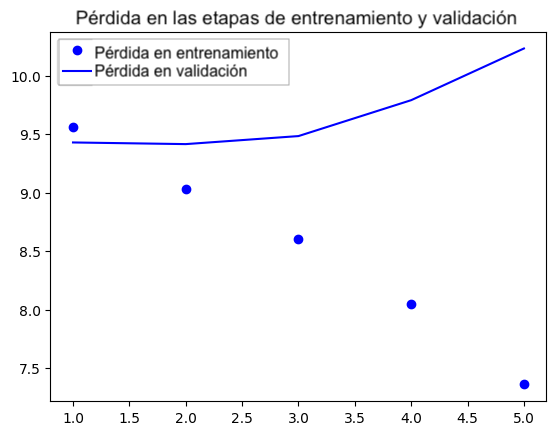
\includegraphics[width=\textwidth]{assets/clasica.png}
		\caption{Modelo Clásico}
		\label{fig:sub1}
	\end{subfigure}
	\hfill
	\begin{subfigure}[b]{0.45\textwidth}
		\centering
		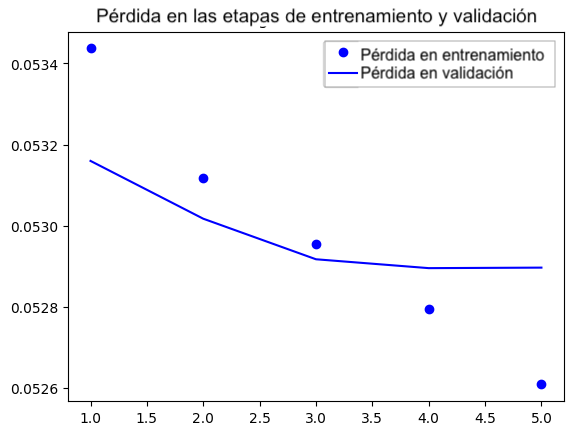
\includegraphics[width=\textwidth]{assets/propuesta.png}
		\caption{Modelo Propuesto}
		\label{fig:sub2}
	\end{subfigure}
	\caption{Dos subimágenes en una figura}
	\label{fig:imagen_completa}
\end{figure}

Antes de llegar a la concepción final del modelo, se consideraron varias modificaciones en los hiperparámetros, como el número de capas, la cantidad de unidades por capa, el número de épocas (reentrenamientos) y el tamaño de lote (\textit{batch size}). Inicialmente, las métricas arrojaban valores poco realistas, lo que reflejaba la inexperiencia del equipo en el tema de aprendizaje automático. Todos esta modificaciones y sus resultados se pueden observar en la tabla \ref{tab:comparacion_modelos}.


\begin{table}[h!]
	\centering
	\begin{tabular}{|c|p{2.5cm}|c|c|p{1.8cm}|p{2.8cm}|}
		\hline
		\textbf{Versión} & \textbf{Arquitectura} & \textbf{Épocas (e)} & \textbf{Tamaño del Lote (b)} & \textbf{Prueba de Pérdida \newline (MSE)} & \textbf{ Accuracy / \newline MAE / MSE de Prueba} \\ \hline
		1 & SimpleRNN(128) & 20 & 20 & 6.2698e-05 & 0.00092908 \\ \hline
		2 & SimpleRNN(512) & 20 & 20 & 0.00034988 & 11416425.0 \\ \hline
		3 & SimpleRNN(512) & 10 & 15 & 0.00042967 & 0.00930194 \\ \hline
		4 & LSTM(512) & 10 & 15 & 6.3452e-05 & 0.00046207 \\ \hline
		5 & GRU(512) & 10 & 15 & 6.2358e-05 & 0.00031208 \\ \hline
		6 & GRU(512) + \newline SimpleRNN(128) & 10 & 15 & 6.2331e-05 & 0.00036732 \\ \hline
		7 & GRU(512) + \newline SimpleRNN(128) & 10 & 15 & 6.3473e-05 & 0.00050875 \\ \hline
		8 & GRU(512) & 10 & 15 & 0.0423731 & 0.16098939 (MAE) \\ \hline
		9 & GRU(512) + \newline SimpleRNN(128) & 10 & 15 & 0.0432334 & 0.16354895 (MAE) \\ \hline
		10 & 2xLSTM(312) + \newline Dropout(0.3) & 10 & 32 & 0.0201351 & 0.15644987 (MAE), 0.04027072 (MSE) \\ \hline
		11 & 2xLSTM(312) + \newline Dropout(0.3) + \newline EarlyStop & 10 & 32 & 0.0201255 & 0.15671074 (MAE), 0.04025150 (MSE) \\ \hline
		12 & GRU(312) + \newline LSTM(312) + \newline Dropout(0.3) + \newline EarlyStop & 10 & 32 & 0.0201129 & 0.15647839 (MAE), 0.04022629 (MSE) \\ \hline
		13 & GRU(312) + \newline Dense(312) + \newline LSTM(624) & 10 & 32 & 0.0201110 & 0.15653566 (MAE), 0.04022256 (MSE) \\ \hline
		14 & GRU(312) + \newline LSTM(312) + \newline Dropout(0.3) & 10 & 20 & 0.0201055 & 0.15649308 (MAE), 0.04021137 (MSE) \\ \hline
	\end{tabular}
	\caption{Comparación de resultados de distintas versiones de modelos}
	\label{tab:comparacion_modelos}
\end{table}


\section{Conclusión}

En este trabajo se entrenaron varias implementaciones de redes neuronales recurrentes para conformar un sistema de recomendaciones secuencial de productos de bellezas a usuarios basadas en sus interacciones. Aunque los resultados de los modelos implementados no fueron nada buenos con respecto a muchos de los trabajos similares existentes \cite{hidasi2015session,chung2014empirical,tang2018personalized} el sistema de recomendación recomienda artículos que empíricamente el equipo considera que pueden interesarles según las compras de prueba que efectuaron.

Es muy importante destacar que este proyecto no solo consistió únicamente en la creación del modelo de ML, sino en todo el proceso entero: desde la construcción y limpieza de los conjuntos de datos así, como la idea de la propuesta innovadora, como el modelado de cada red neuronal. Por lo tanto, sirvió también para ganar experiencias en la construcción de sistemas de recomendación, y comprender aún más lo tan variado que son los sistemas de recuperación de información.

Para futuros trabajos similares a este se sugieren las siguientes recomendaciones:
\begin{itemize}
	\item De ser posible, emplear conjuntos de datos con mayor diversidad y cantidad para mejorar la capacidad del modelo de generalizar.
	\item Entrenar múltiples redes neuronales utilizando secuencias de diferentes longitudes y luego integrarlas en un solo modelo capaz de procesar entradas de variados tamaños, lo que podría aumentar la flexibilidad y precisión del sistema de recomendación.
	\item Incorporar datos de una gama más amplia de productos, como electrodomésticos, productos de belleza, artículos de aseo personal, ropa y accesorios, herramientas, entre otros. Esto permitiría un embedding de productos más diverso, con una mayor proximidad entre productos de la misma categoría, lo que enriquecería las recomendaciones.
	\item Considerar el entrenamiento de redes neuronales con un mayor número de nodos por capa para capturar de manera más efectiva las complejidades en los datos. Dado que esto requiere un considerable poder de cómputo, se recomienda utilizar plataformas en la nube más potentes que el plan gratuito de Google Colab.
\end{itemize}

\bibliographystyle{plain}
\bibliography{assets/biblio.bib}

\end{document}
